\documentclass[letterpaper,10pt,titlepage,fleqn]{article}

%example of setting the fleqn parameter to the article class -- the below sets the offset from flush left (fl)
\setlength{\mathindent}{1cm}

\usepackage{graphicx}                                        
\usepackage{amssymb}                                         
\usepackage{amsmath}                                         
\usepackage{amsthm} 
\usepackage{esint}
\usepackage{nopageno}
\usepackage{booktabs}                            
\usepackage{alltt}                                           
\usepackage{float}
\usepackage{color}
\usepackage{fancyhdr}
\usepackage{url}
\usepackage{balance}
\usepackage[TABBOTCAP, tight]{subfigure}
\usepackage{enumitem}
\usepackage{pstricks, pst-node}
%the following sets the geometry of the page
\usepackage{geometry}
\geometry{textheight=9in, textwidth=6.5in}
\pagestyle{fancy}
% random comment
\newcommand{\cred}[1]{{\color{red}#1}}
\newcommand{\cblue}[1]{{\color{blue}#1}}
\usepackage{hyperref}
\usepackage{textcomp}
\usepackage{listings}
\def\name{Best CS325 Group}
%% The following metadata will show up in the PDF properties
\hypersetup{
  colorlinks = true,
  urlcolor = black,
  pdfauthor = {\name},
  pdfkeywords = {cs311 ``operating systems'' files filesystem I/O},
  pdftitle = {Pertinent Information},
  pdfsubject = {Virtual Reality Lab},
  pdfpagemode = UseNone
}

\parindent = 0.0 in
\parskip = 0.2 in
\fboxsep=5mm%padding thickness
\fboxrule=4pt%border thickness

\begin{document}
\lstset{language=Python} 

\title{Programming Assignment \#1 - CS325}

\author{
	Joshua Villwock \and
	Jaron Thatcher \and
	Ryan Phillips
}

\date{January 31, 2014}
\maketitle
%to remove page numbers, set the page style to empty
\section*{Introduction}
\hrule

Inversion counting is a common problem in computer science. In this document, we will present three different algorithms to solve the issue. Also included are proofs for the algorithms, as well as empirical and asymptotic analysis of their run time on increasingly sized inputs.


\section*{Pseudocode}
\hrule
\begin{centering}

\textbf{Brute Force:}
\end{centering}
\begin{lstlisting}
BruteForce(arr)
  count = 0
  for i in 0 to arr.length
    for j in i to arr.length
	if arr[i] > arr[j]:
        count++ 
  return count
\end{lstlisting}

\begin{centering}
\textbf{Naive Divide and Conquer:}
\end{centering}
\begin{lstlisting}
NaiveDivideAndConquer(arr)
  count = 0
  if len(arr) < 2:
    return count
  middle = length(list_in)/2
  left = arr[:middle] // slice off half of the array
  right = arr[middle:]
  // count inversions between left and right halves
  for i in range (0,len(left)):
    for j in range (0,len(right)):
      if left[i] > right[j]:
	  count++
  // and count internal inversions recursively
  count += NaiveDivideAndConquer(left)
  count += NaiveDivideAndConquer(right)
  return count
\end{lstlisting}

\begin{centering}
\textbf{Merge and Count:}
\end{centering}

\begin{lstlisting}
MergeAndCount(arr,0)
  results = []
  // base case
  if len(x) < 2:
    return x, count
  middle =len(x)/2
  // recursive calls
  left, count = MergeAndCount(x[:middle],count)
  right, count = MergeAndCount(x[middle:],count)
  i, j = 0, 0
  while i < length(left) and j < length(right):
    if left[i] > right[j]:
      results.append(right[j])
      count += length(left) - i
      j++
    else:
      results.append(left[i])
      i++
    results += left[i:]
    results += right[j:]
    return results, count
\end{lstlisting}

\section*{Correctness Proofs}
\hrule

\begin{centering}
\textbf{Naive Divide and Conquer:}
\end{centering}

\begin{centering}
\textbf{Merge and Count:}
\end{centering}

Pre-explanation:

Merge \& Count works by simply running mergesort on the list, and counting how many times elements are inverted.  Mergesort works (code actually flows in the other direction, as it is recursive, however it makes more sense conceptually this way) by splitting the Length N list into n separate elements, then continues to combine those into n/2 lists of 2n length.  It does this by comparing the existing ``lists'' (singlets) and moving the smallest of the first elements of either list into the new list, thereby sorting them.

Proof by contradiction:

Assume that one of the resulting lists is incorrect.  If one of the lists obtained by combining smaller lists was not sorted, then mergesort would no longer work, and therefore the inversion counting would also be incorrect.  The only way for this to happen is for the smaller sub-lists to be incorrectly sorted, (since we assume they are sorted, and only look at the first elements in either) and the only way for those to be incorrectly sorted is if exactly what we are talking about right now is true.  Eventually we get to the base case, where each sub-list is only 1 element, but it is impossible to mess this up, since there is no way for a single-element list to not be sorted.

\section*{Asymptotic Analysis of Run Time}
\hrule
\begin{centering}
\textbf{Brute Force:}
\end{centering}
It uses two nested loops, with the lower bound of the inner set to the current value of the outer. 

\begin{lstlisting}
This has a runtime of: 

(n^2 + n) / 2 

Which can also be expressed as:

O(n^2)
\end{lstlisting}

\begin{centering}
\textbf{Naive Divide and Conquer:}
\end{centering}

\begin{lstlisting}

Recurrence Relation:

T(n) = O(n/2)^2 + 2T(n/2)
T(n) = (n^2)/4 + 2T(n/2) // 1st

Telescoping: 

T(n/2) = ((n/2)^2 / 4) + 2T(n/4) = n^2 / 16 + 2T(n/4) // 2nd

General form:

T(n) = (1/2)*(-1+n)n + (n + c)/2

Since we have the following terms: (1/2)*n^2 + (1/2)n

This can be simplified as just: O(n^2)

\end{lstlisting}

\begin{centering}
\textbf{Merge and Count:}
\end{centering}

\begin{lstlisting}
T(n) = T(n/2) + O(n) 
T(n) = T(n/2) + cn // 1st recursion 

Telescoping:

[T(n/4) + cn] + cn = T(n/4) + 2cn // 2 
[T(n/8) + cn] + 2cn = T(n/8) = 3cn // 3 

General Pattern: T(n/2^n) + ncn

When T(n) = T(n/(2^n) + ncn

You have two subproblems of size n
Plus linear time combination

AKA: O(n log n)
\end{lstlisting}

\section*{Testing}
\hrule
The first test for correctness was performed using the provided file ``verify.txt''. It was assumed that the last value of each row was the expected number of inversions, so all 3 algorithms were run on each row of values (excluding the last), and this was compared to the expected value. This can be performed via: ``test\_correctness1(``verify.txt'')''.

The second test for correctness used the second provided file ``test\_in.txt''. Since no expected values were given, the results were just printed out. All 3 algorithms gave the same value, so this is a good indication. The results have been included below, with just a single value given (number of inversions) for each row in the test file. This test can be run by calling the function ``test\_correctness2(``test\_in.txt'')''.

Results:
252180, 250488, 243785, 247021, 250925, 256485, 249876, 253356, 255204, 247071

\section*{Extrapolation and Interpretation}
\hrule

\begin{centering}
\textbf{Slope of lines in log-log plot:}
\end{centering}

The equation for the best fit line on the log-log plot (calculated using numpy.polyfit()) has the following form:

f(n) = e\textsuperscript{y-intercept} * n\textsuperscript{slope}

Brute Force:
\begin{itemize}
\item slope: 2.05692581355
\item y-intercept: -17.5588327907
\end{itemize}

Naive Divide \& Conquer:
\begin{itemize}
\item slope: 2.03626014268
\item y-intercept: -17.3982172216
\end{itemize}

Merge \& Count:
\begin{itemize}
\item slope: 1.10025742067
\item y-intercept: -13.1947528938
\end{itemize}

\begin{centering}
\textbf{Largest input item solvable in an hour:}
\end{centering}

Extrapolation using the best fit function from the previous section: 

f(n) = Runtime = 1 hr = e\textsuperscript{y-intercept} * n\textsuperscript{slope}

Solving for n, using the values from the above chart, yields the following numbers: 

Brute Force: 265410

Naive Divide \& Conquer: 299864

Merge \& Count: 275733290

\begin{centering}
\textbf{Discrepancy between actual and asymptotic:}
\end{centering}

The slopes of the first two best fit lines on the log-log graph are very close to 2, and the third is just over 1.1. This matches up with what is expected - i.e. there is no real discrepency to report.

\newpage

\section*{Empirical Analysis of Run Time}
\hrule
\textbf{Linear Plot:}
\vskip 0.04in
\begin{center}
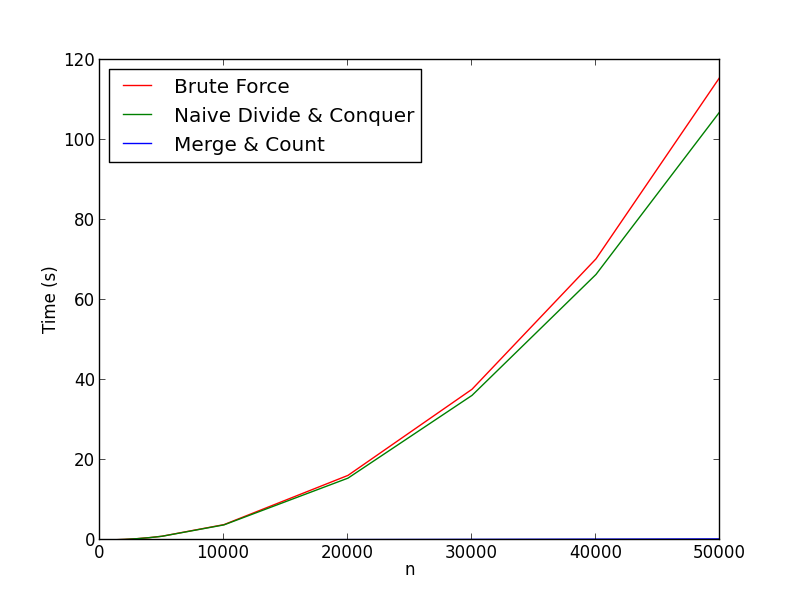
\includegraphics[width=4.5in]{input_time.png}
\end{center}
\textbf{Log-log Plot:}
\vskip 0.04in
\begin{center}
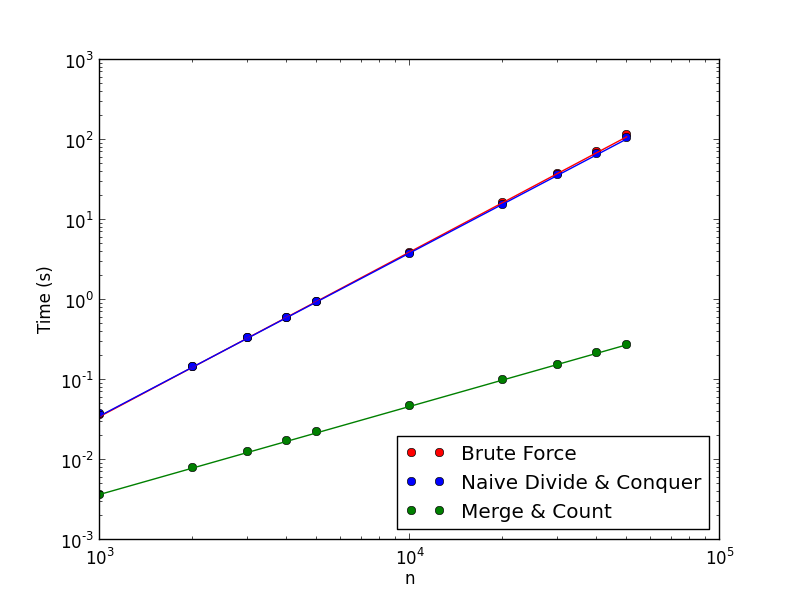
\includegraphics[width=4.5in]{loglog.png}
\end{center}
\end{document}
